\section{Consonância}
\index{Música!Consonância}
\label{sec:consonancia}

\begin{tcbinformation} 
\textbf{Consonância:}
\index{Música!Consonância}
\label{ref:consonancia}

Relação de sons agradáveis ao ouvido.

\end{tcbinformation} 


A escola Pitagórica que existiu no seculo VI A.C.,
tentava compreender o universo, e
com esse fim desenharam modelos matemáticos para explicar 
os fenômenos observados;
entre os temas que foram tratados estava incluída a música,
e porque alguns conjuntos de sons eram mais 
agradáveis de ouvir que outros \cite[pp. 11]{arbones2012armonia}.

Nos trabalhos feitos pela escola pitagórica, 
está incluído a criação de um instrumento chamado monocórdio;
este consta de uma única corda,
que tem um delimitador para modificar a longitude sem alterar a tensão nela \cite[pp. 12]{arbones2012armonia},
de modo que quando a corda do monocórdio é exitada o instrumento produz um som;
na Figura \ref{fig:consonancia}a podemos ver um modelo do monocórdio com a corda completa, 
que gera um som com frequência ``f''.
\begin{figure}[!h]
  \centering
    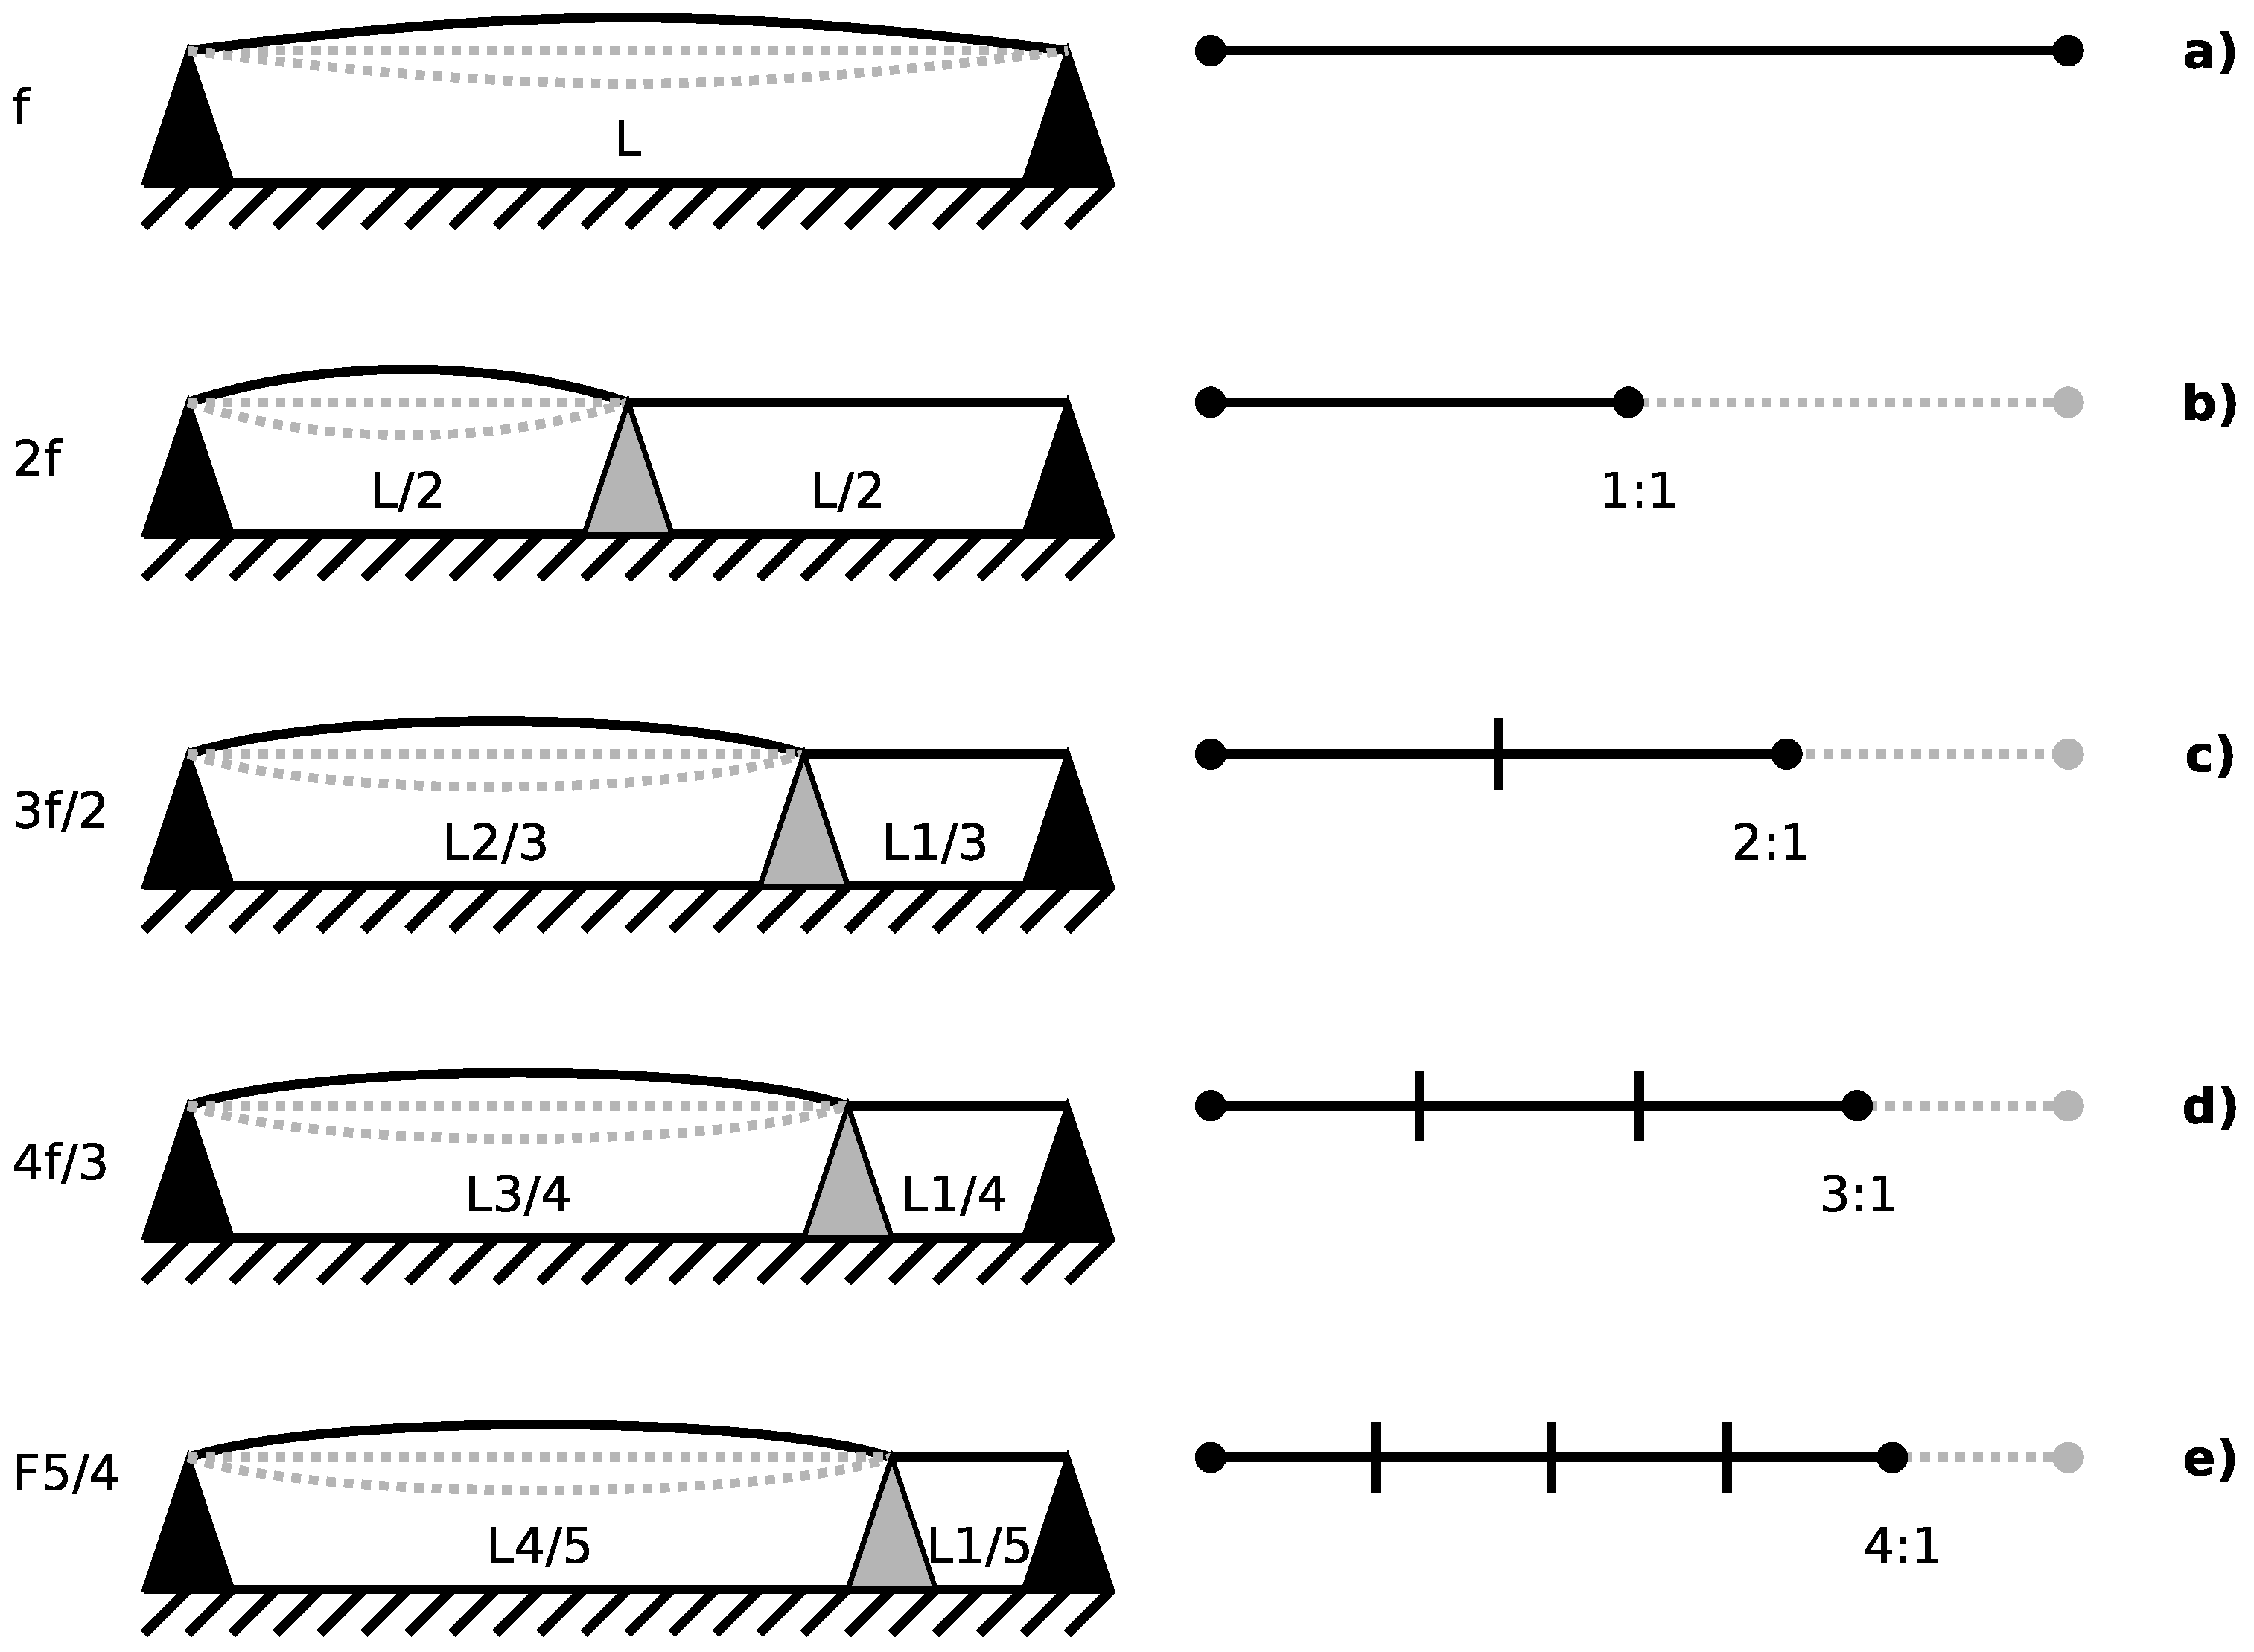
\includegraphics[width=\textwidth]{chapters/cap-musica-composer/consonancia0.eps}
\caption{Consonância entre frequências.}
\label{fig:consonancia}
\end{figure}

Quando a longitude da corda do monocórdio diminui, 
a frequência do som gerado aumenta, é dizer se obtêm tons mais agudos,
tendo longitude e frequência uma relação inversa \cite[pp. 12]{arbones2012armonia}. 
Entre os resultados obtidos com este instrumento, 
está a constatação de que algumas longitudes menores da corda, 
geravam sons mais agradáveis de ouvir, ao ser executados ao mesmo tempo com o som gerado pela corda completa \cite[pp. 12]{arbones2012armonia}.

Assim, os pitagóricos descobriram que as proporções mais simples das cordas,
eram as que geravam os sons mais agradáveis de ouvir \cite[pp. 12]{arbones2012armonia};
nas Figuras \ref{fig:consonancia}[b - e], podemos ver algumas das proporções de longitudes estudadas,
como: 1:1, 2:1, 3:1 e 4:1; que geram tons com frequências: 
$2$f, $\frac{3}{2}$f, $\frac{4}{3}$f e , $\frac{5}{4}$f.
Sendo a relação mais simples (1:1) a que provoca a duplicação da frequência (Figura \ref{fig:consonancia}b),
que na atualidade chamamos \hyperref[sec:pos:Oitava]{\textbf{oitava}}; 
a seguinte em simplicidade é a proporção 2:1 que gera um som com uma frequência de $\frac{3}{2}$f (Figura \ref{fig:consonancia}c),
que na atualidade chamamos de \textbf{intervalo de quinta};
por outro lado, nas Figuras \ref{fig:consonancia}[d-e] com frequências $\frac{4}{3}$f e , $\frac{5}{4}$f respetivamente,
a sensação de consonância diminui proporcionalmente à complexidade das frações na frequencia \cite[pp. 12]{arbones2012armonia}.

Por estas observações os pitagóricos concluíram que seriam consonantes com a frequência $f$, sons com uma frequência igual a 
\begin{equation}
\label{eq:simplespita}
\frac{n+1}{n}f,
\end{equation}
sendo que o nível de consonância diminui com o aumento de ``n'' \cite[pp. 14]{arbones2012armonia}.

\PRLsep{Escala diatônica}
\label{ref:paginadiatonicanumerica}

Se usamos as frequências da Equação \ref{eq:simplespita}, para $n=\{1,2,3,4\}$,
e multiplicamos estas frequências por $\frac{3}{2}$ ou $\frac{1}{2}$, que
são as proporções de frequência que geram maior consonância,
obteremos a \hyperref[sec:pos:Diatonica]{\textbf{escala diatônica}} (E.D.).
Esta escala pode ser comparada com a \hyperref[sec:pos:Cromatica]{\textbf{escala cromática}} (E.C.)
que está \hyperref[subsec:tempigual]{\textbf{igualmente temperada}}, 
como mostra a Tabela \ref{tab:pitagorascromatica}, onde foi usada a nota musical ``dó'' como referencia, a \hyperref[sec:Tonica]{\textbf{tônica}}.
\begin{table}[h]
  \centering
  \begin{tabular}{|l|l|l|l|l|l|l|l|l|}
  \hline
  E. Diatônica  & dó & ré & mi & fá & sol & lá & si & dó \\ \hline
  \hline
  Freq. E.D.  & f  & $\frac{9}{8}$f & $\frac{5}{4}$f & $\frac{4}{3}$f & $\mathbf{\frac{3}{2}}$\textbf{f} & $\frac{5}{3}$f & $\frac{15}{8}$f & $\mathbf{2}$\textbf{f}\\ \hline
  E. Cromática & f  & $\alpha^{2}$f  & $\alpha^{4}$f  & $\alpha^{5}$f  & $\alpha^{7}$f  & $\alpha^{9}$f  & $\alpha^{11}$f  & $2$f\\ \hline \hline
  Error$\%$ &  0.0 & 0.23 & 0.79 & 0.11 & 0.11 & 0.91 & 0.68 & 0.0 \\ \hline
  \end{tabular}
  \caption{Relação de frequências, usando $\alpha=2^\frac{1}{12}$.}
  \label{tab:pitagorascromatica}
\end{table}

É possível ver que existe uma ligeira diferença numérica, 
entre as proporções de frequências na escala diatônica baseada nas consonâncias descobertas pela escola pitagórica,
e as proporções de frequência de nossa atual escala cromática igualmente temperada,
no menor dos casos temos um $0.11\%$ de erro na frequência, 
e no pior dos casos menos de um $1\%$ de diferença\footnote{Para ter uma referencia,
é interessante lembrar que se precisa de um incremento de $5.9463\%$ na frequência, 
para subir um semitom na escala cromática igualmente temperada.}.

\PRLsep{Análises objetivo}
Fora da subjetiva perspetiva da escola pitagórica em indicar que, 
frações mais simples na frequência, 
geram sons consonantes; 
existem motivos objetivos para fundamentar esta afirmação.

Na Figura \ref{fig:corda32} podemos ver as sinais $y_{f}$ e $y_{\frac{3}{2}f}$, 
produzidas pelos sons com frequências $f=1000$hz e $\frac{3}{2}f$,
correspondentes a cordas de longitude $L$ e $\frac{2}{3}L$ respetivamente;
é interessante observar que se precisam \textbf{dois} ciclos completos da sinal $y_{f}$,
para que ambas sinais voltem a estar em sincronia e que a sinal soma, $y_{f}+y_{\frac{3}{2}f}$, forme um ciclo completo.


Nesse sentido, na Figura \ref{fig:corda53} podemos observar as sinais $y_{f}$ e $y_{\frac{5}{3}f}$, 
produzidas pelos sons com frequências $f=1000$hz e $\frac{5}{3}f$,
correspondentes a cordas de longitude $L$ e $\frac{3}{5}L$ respetivamente;
e similarmente ao caso anterior, observamos que se precisam \textbf{três} ciclos completos da sinal $y_{f}$,
para que ambas sinais voltem a estar em sincronia e que a sinal soma, $y_{f}+y_{\frac{5}{3}f}$, forme um ciclo completo.

\begin{figure}
    \centering
    \begin{subfigure}[b]{0.6\textwidth}
        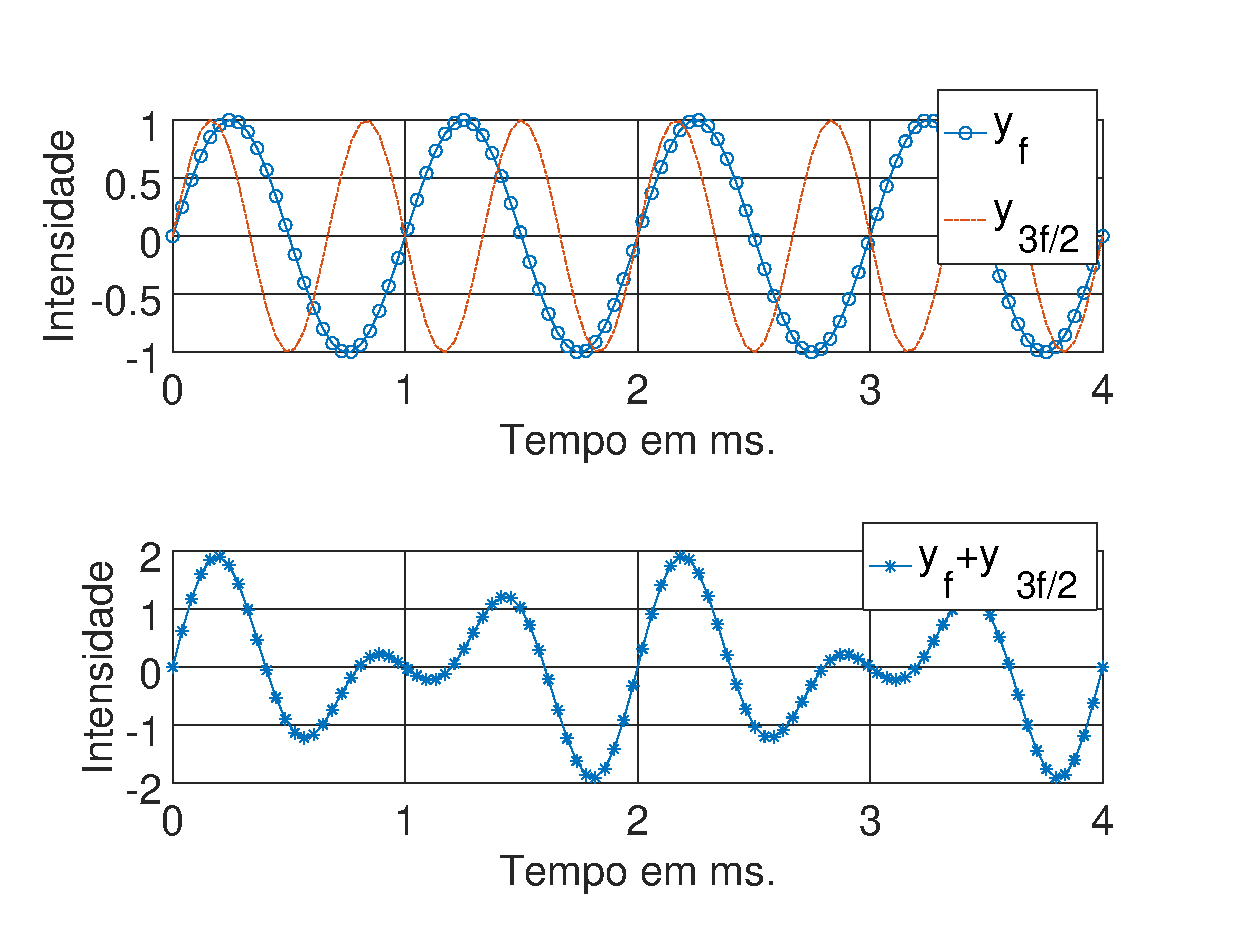
\includegraphics[width=\textwidth]{chapters/cap-musica-composer/consonancia32.eps}
        \caption{Consonância entre sinais com frequências $f$ e $\frac{3}{2}f$}
        \label{fig:corda32}
    \end{subfigure}
    ~ %add desired spacing between images, e. g. ~, \quad, \qquad, \hfill etc. 
      %(or a blank line to force the subfigure onto a new line)
    \begin{subfigure}[b]{0.6\textwidth}
        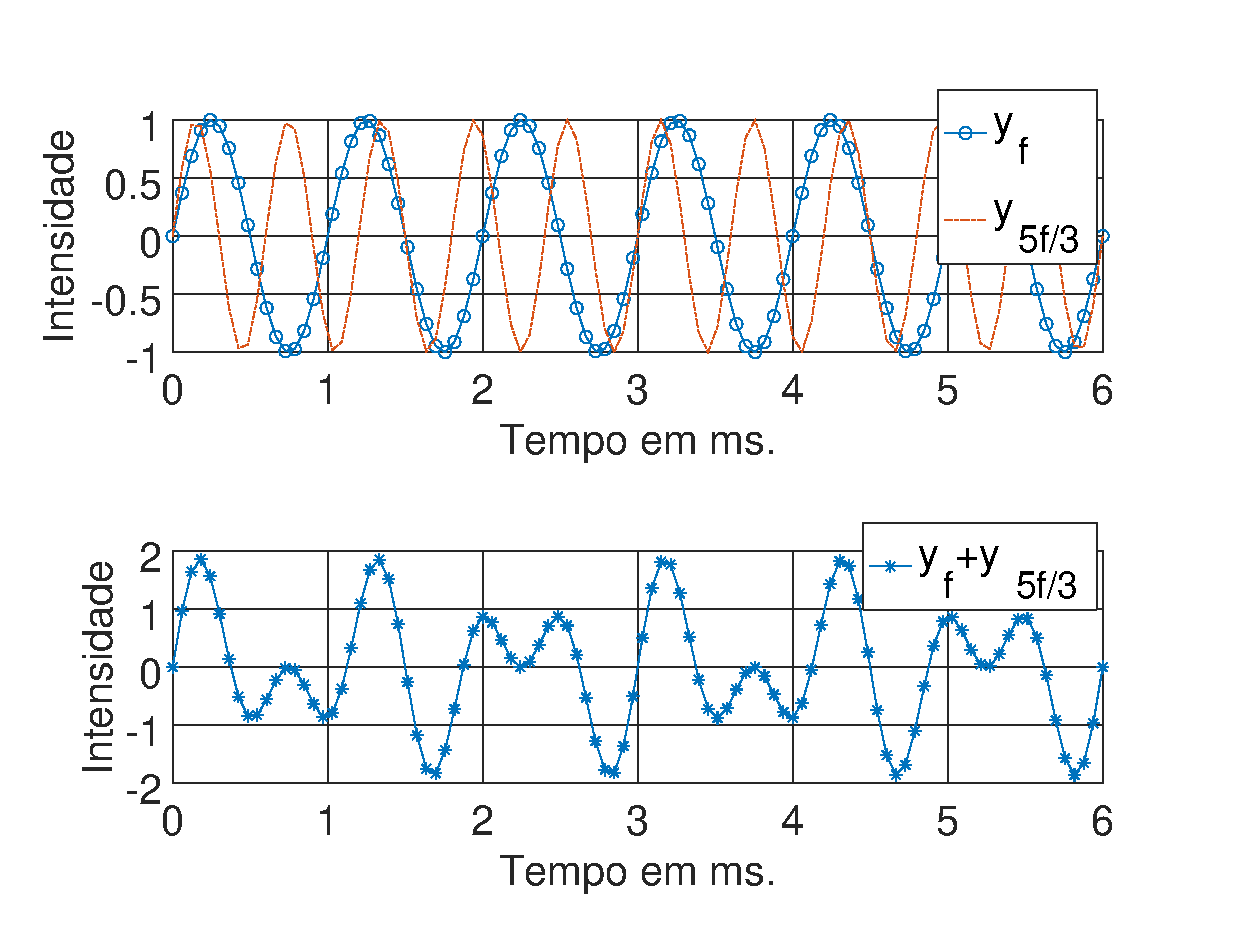
\includegraphics[width=\textwidth]{chapters/cap-musica-composer/consonancia53.eps}
        \caption{Consonância entre sinais com frequências $f$ e $\frac{5}{3}f$}
        \label{fig:corda53}
    \end{subfigure}
\caption{Analises de consonância.}
\label{fig:consonanciaper}
\end{figure}

Assim, deduzimos que pela forma fraccionaria e relativa das frequência nas sinais, 
podemos usar o denominador da fração na frequência,
para conhecer quantos ciclos debem passar para que a ambas sinais em estudo voltem a estar em sincronia;
de modo que seremos capazes de relacionar um estado de maior nível de consonância (N.C.) a um menor numero de ciclos.
A Tabela \ref{tab:pitagorascromatica2} mostra estas relações, 
porem foram agregadas as letras ``a'' e ``b'' para indicar maior e menor consonância respetivamente,
nos casos com igual N.C., este critério foi aplicado tomando em conta que a escala
que comumente temos num piano está igualmente temperada,
é como vimos na Tabela  \ref{tab:pitagorascromatica},
existe um erro de aproximação a estas frações;
de modo que foi colocada a etiqueta de ``b'' ao caso de maior erro e a etiqueta de ``a'' ao de menor.
\begin{table}[h]
  \centering
  \begin{tabular}{|l|l|l|l|l|l|l|l|l|}
  \hline
  E. Diatônica    & dó & ré & mi & fá & sol & lá & si & dó \\ \hline
  \hline
  Semitons E.C.   & 0  & 2  & 4  & 5  & 7  & 9  & 11 & 12 \\ \hline
  Freq. E.D.  & f  & $\frac{9}{8}$f & $\frac{5}{4}$f & $\frac{4}{3}$f & $\mathbf{\frac{3}{2}}$\textbf{f} & $\frac{5}{3}$f & $\frac{15}{8}$f & $\mathbf{2}$\textbf{f}\\ \hline \hline
  N.C. &  0 & 8a & 4 & 3a & 2 & 3b & 8b & 1 \\ \hline
  \end{tabular}
  \caption{Nível de consonância com a nota musical dó.}
  \label{tab:pitagorascromatica2}
\end{table}

\begin{example}
Com a ajuda de um piano, que esteja igualmente temperado,
use a nota dó como referencia e comprove o nível de consonância com todas as demais notas musicais;
verifique se concorda com o mostrado na Tabela \ref{tab:pitagorascromatica2}.
\end{example}

\PRLsep{Conclusões}

Podemos concluir que existe uma maior consonância entre
\begin{itemize} 
\item os tons com frequências $f$ e $2f$, e 
\item os tons com frequências $f$ e $\frac{3}{2}f$;
\end{itemize}
com outros valores de frequência, 
como entre $f$ e $\frac{4}{3}f$, o nível de consonância diminui  
 gradualmente com o aumento da complexidade das frações nas frequências.

Na música atual, as relações de consonância são usadas na escala cromática, 
em notas musicais com:
\begin{itemize} 
\item Uma oitava de diferença, para as frequências relacionadas como $f$ e $2f$, 
por exemplo: dó e dó'.
\item Um intervalo de quinta, sete semitons, para frequências relacionadas como  $f$ e $\frac{3}{2}f$, 
por exemplo: dó e sol. Porem, numa escala igualmente temperada, 
os 7 semitons são uma aproximação\footnote{Sim, você está supondo certo,
toda a música atual está ligeiramente ``desafina'', pois usa uma aproximação para a consonância.}
 da fração $\frac{3}{2}$.
\end{itemize}

